%!TEX root = ../thesis.tex
\section{部品の製作}
本研究で製作したロボットアームには,3Dプリント部品と板金部品を使用した.3Dプリント部品は,FDM方式の3Dプリンタを用いて製作した(図\ref{fig:3Dprint}参照).一方,板金部品については,ミスミ株式会社が提供する板金・機械加工のオンライン外注サービス「meviy」\cite{meviy:online}を利用して外注製作を行った(図\ref{fig:meviy}参照).このサービスの利用により,専門的な加工技術を持たない場合でも,短納期で部品を調達することが可能である.

その他の部品については,既製品を採用した.特に,QDDモータ以外の部品はすべてMISUMI\cite{misumi:online}で発注可能な汎用部品を使用した.部品の選定基準は価格,納期,および性能とした.図\ref{fig:parts}に部品リストを示す.
\begin{figure}
  \centering
  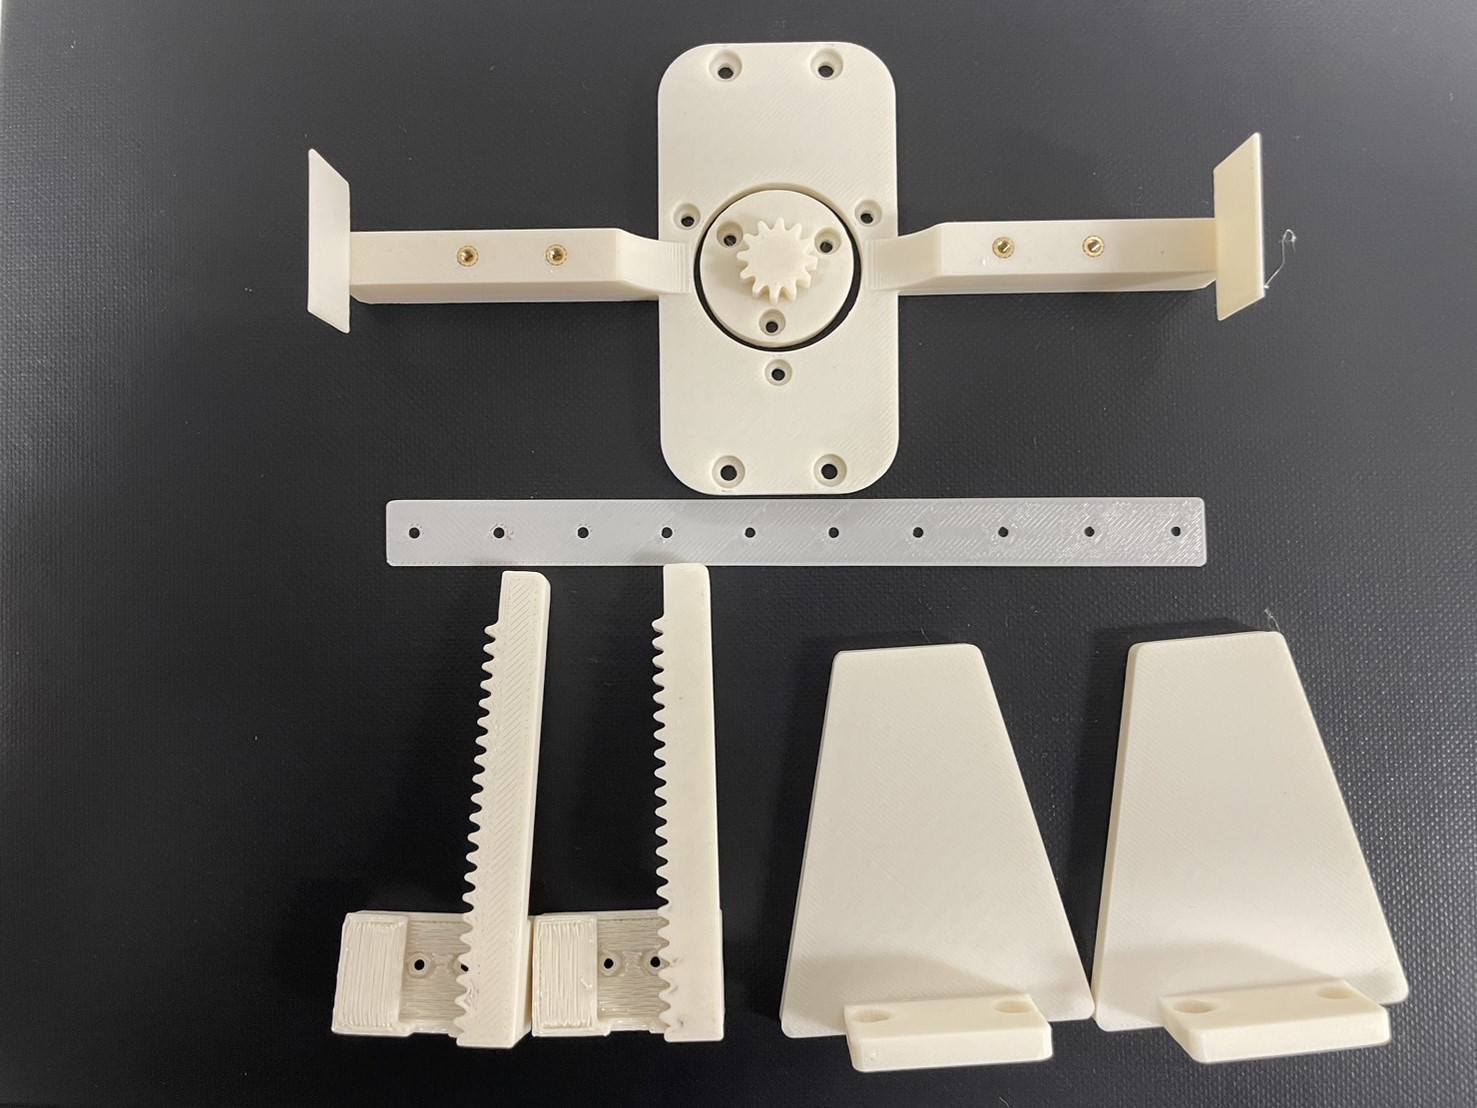
\includegraphics[width=10cm]{images/product/3Dprint.jpg}
  \caption{3D printed parts}
  \label{fig:3Dprint}
\end{figure}
\begin{figure}
  \centering
  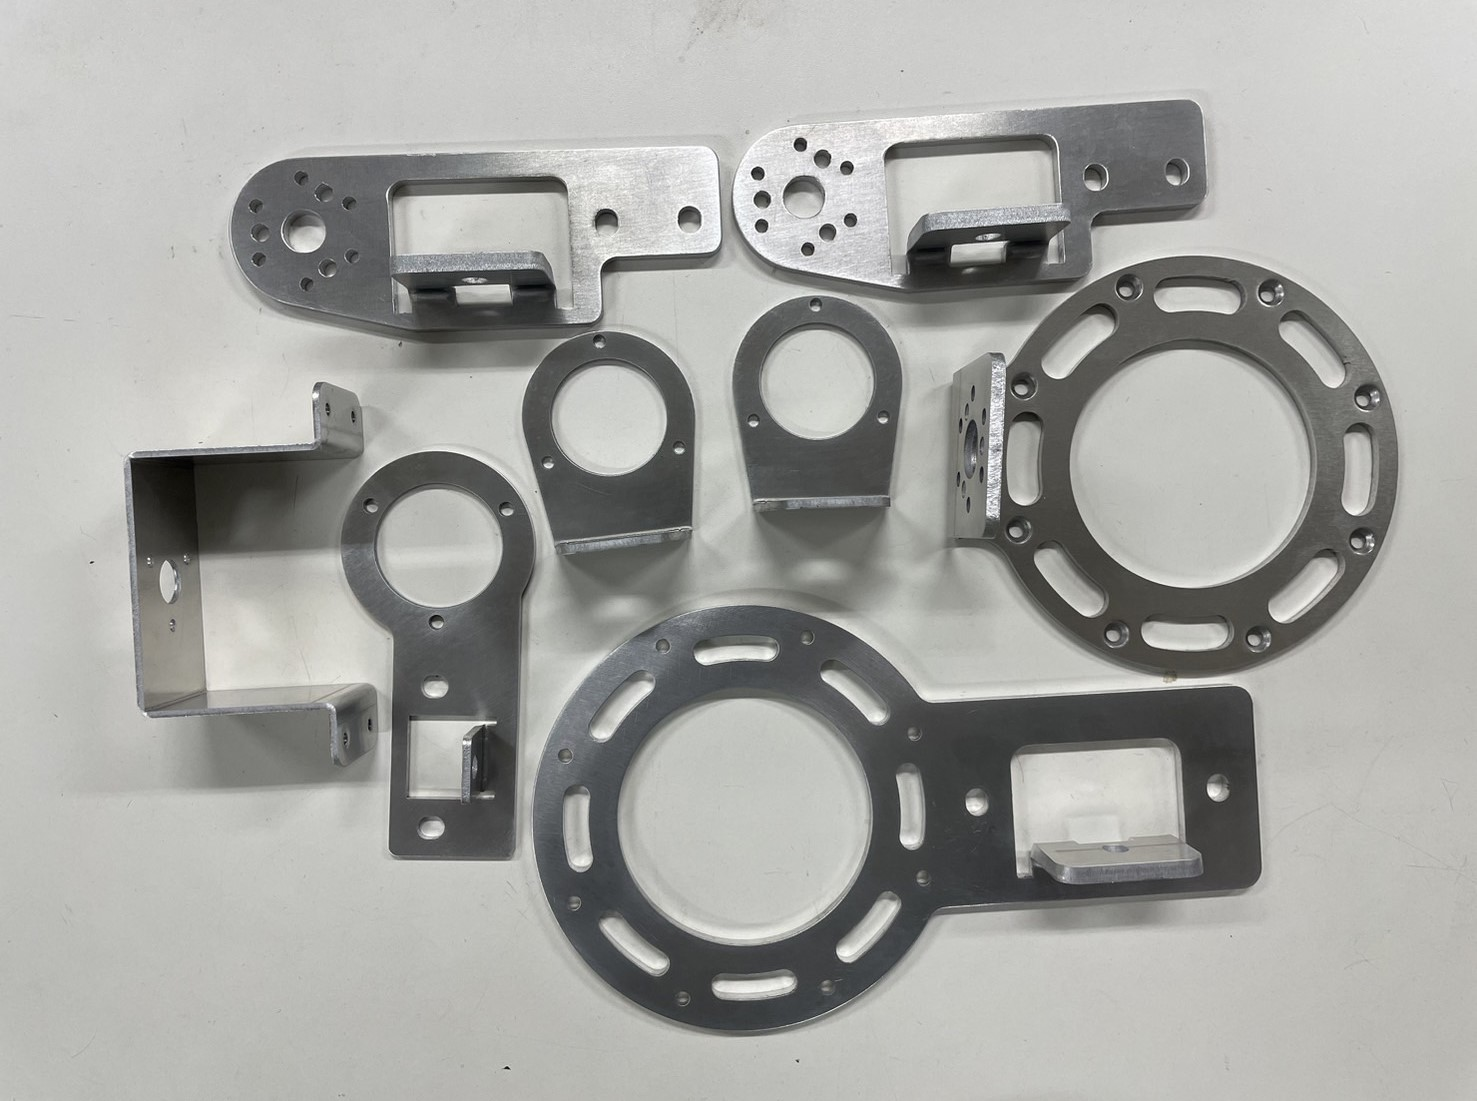
\includegraphics[width=10cm]{images/product/meviy.jpg}
  \caption{Parts ordered from Meviy}
  \label{fig:meviy}
\end{figure}
\begin{figure}
  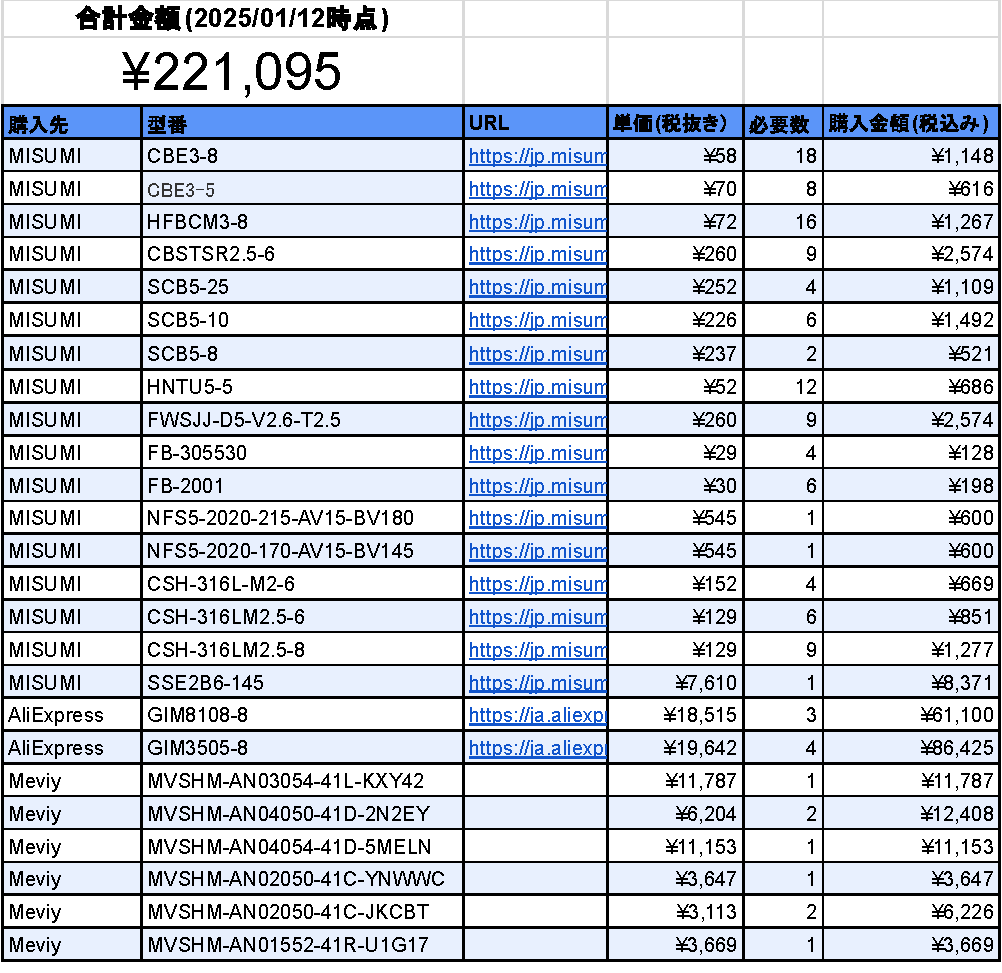
\includegraphics[width=14cm]{images/product/list.pdf}
  \caption{Parts list}
  \label{fig:parts}
\end{figure}
\clearpage
\newpage